\documentclass{article}

\usepackage{color}
\usepackage{listings}
\usepackage{fullpage}
\usepackage{graphicx}

\definecolor{gray_ulisses}{gray}{0.55}
\definecolor{castanho_ulisses}{rgb}{0.71,0.33,0.14}
\definecolor{preto_ulisses}{rgb}{0.41,0.20,0.04}
\definecolor{green_ulises}{rgb}{0.2,0.75,0}

\lstdefinelanguage{HaskellUlisses}
{
	basicstyle=\ttfamily\scriptsize,
	%backgroundcolor=\color{yellow},
	%frameshape={RYRYNYYYY}{yny}{yny}{RYRYNYYYY}, %contornos... muito nice...
	sensitive=true,
	morecomment=[l][\color{gray_ulisses}\scriptsize]{--},
	morecomment=[s][\color{gray_ulisses}\scriptsize]{\{-}{-\}},
	morestring=[b]",
	stringstyle=\color{red},
	showstringspaces=false,
	numbers=none,
	firstnumber=\thelstnumber,
	numberstyle=\tiny,
	numberblanklines=true,
	showspaces=false,
	showtabs=false,
	xleftmargin=15pt,
	xrightmargin=-20pt,
	emph=
	{[1]
		FilePath,IOError,abs,acos,acosh,all,and,any,appendFile,approxRational,asTypeOf,asin,
		asinh,atan,atan2,atanh,basicIORun,break,catch,ceiling,chr,compare,concat,concatMap,
		const,cos,cosh,curry,cycle,decodeFloat,denominator,digitToInt,div,divMod,drop,
		dropWhile,either,elem,encodeFloat,enumFrom,enumFromThen,enumFromThenTo,enumFromTo,
		error,even,exp,exponent,fail,filter,flip,floatDigits,floatRadix,floatRange,floor,
		fmap,foldl,foldl1,foldr,foldr1,fromDouble,fromEnum,fromInt,fromInteger,fromIntegral,
		fromRational,fst,gcd,getChar,getContents,getLine,head,id,inRange,index,init,intToDigit,
		interact,ioError,isAlpha,isAlphaNum,isAscii,isControl,isDenormalized,isDigit,isHexDigit,
		isIEEE,isInfinite,isLower,isNaN,isNegativeZero,isOctDigit,isPrint,isSpace,isUpper,iterate,
		last,lcm,length,lex,lexDigits,lexLitChar,lines,log,logBase,lookup,map,mapM,mapM_,max,
		maxBound,maximum,maybe,min,minBound,minimum,mod,negate,not,notElem,null,numerator,odd,
		or,ord,otherwise,pi,pred,primExitWith,print,product,properFraction,putChar,putStr,putStrLn,quot,
		quotRem,range,rangeSize,read,readDec,readFile,readFloat,readHex,readIO,readInt,readList,readLitChar,
		readLn,readOct,readParen,readSigned,reads,readsPrec,realToFrac,recip,rem,repeat,replicate,return,
		reverse,round,scaleFloat,scanl,scanl1,scanr,scanr1,seq,sequence,sequence_,show,showChar,showInt,
		showList,showLitChar,showParen,showSigned,showString,shows,showsPrec,significand,signum,sin,
		sinh,snd,span,splitAt,sqrt,subtract,succ,sum,tail,take,takeWhile,tan,tanh,threadToIOResult,toEnum,
		toInt,toInteger,toLower,toRational,toUpper,truncate,uncurry,undefined,unlines,until,unwords,unzip,
		unzip3,userError,words,writeFile,zip,zip3,zipWith,zipWith3,Impl,Equiv,Prop,Neg,Cnj,Dsj
	},
	emphstyle={[1]\color{blue}},
	emph=
	{[2]
		Bool,Char,Double,Either,Float,IO,Integer,Int,Maybe,Ordering,Rational,Ratio,ReadS,ShowS,String,NoTriangle,Equilateral,Rectangular,Isosceles,Other,Shape
	},
	emphstyle={[2]\color{castanho_ulisses}},
	emph=
	{[3]
		case,class,data,deriving,do,else,if,import,in,infixl,infixr,instance,let,
		module,of,primitive,then,type,where
	},
	emphstyle={[3]\color{preto_ulisses}\textbf},
	emph=
	{[4]
		quot,rem,div,mod,elem,notElem,seq
	},
	emphstyle={[4]\color{castanho_ulisses}\textbf},
	emph=
	{[5]
		EQ,False,GT,Just,LT,Left,Nothing,Right,True,Show,Eq,Ord,Num
	},
	emphstyle={[5]\color{preto_ulisses}\textbf}
}

\lstnewenvironment{code}
{\lstset{language=HaskellUlisses}}
{\smallskip}


\begin{document}
\setlength{\parindent}{0cm}

\title{Software Testing Assignment 2}
\author{Cindy Berghuizen, Omar Pakker , Chiel Peter, Maria Gouseti}
\date{10 September , 2013}
\maketitle
\section*{Triangle Exercise}
\begin{code}
triangle :: Integer -> Integer -> Integer -> Shape
triangle x y z		| (a + b <= c) || (a <1)	= NoTriangle
 			| (a == b && b == c) 		= Equilateral
 			| ((a^2 + b^2) == c^2) 		= Rectangular
 			| (a == b) || (b == c) 		= Isosceles
 			| otherwise			= Other
 			where [a, b, c] = sort [x, y, z]

testTriangle :: Shape -> Integer -> [((Integer, Integer, Integer), Shape)]
testTriangle s maxN = [((a, b, c), s)	| a <- [1..maxN], 
					  b <- [a..maxN], 
					  c <- [b..maxN], 
					  triangle a b c == s]
\end{code}

The function testTriangle takes two input arguments. The first is the type of triangle and the second is the maximum side length. To avoid permutations (b,c) only range over there value of there predecessor and the maximum value as these permutations are mapped to the same values by the sort algortihm inside the triangle function. 10 was chosen as  a maximum value to keep the results acceptable to manual inspection. The results are shown below and where verified to be correct.
\vspace{.3cm}

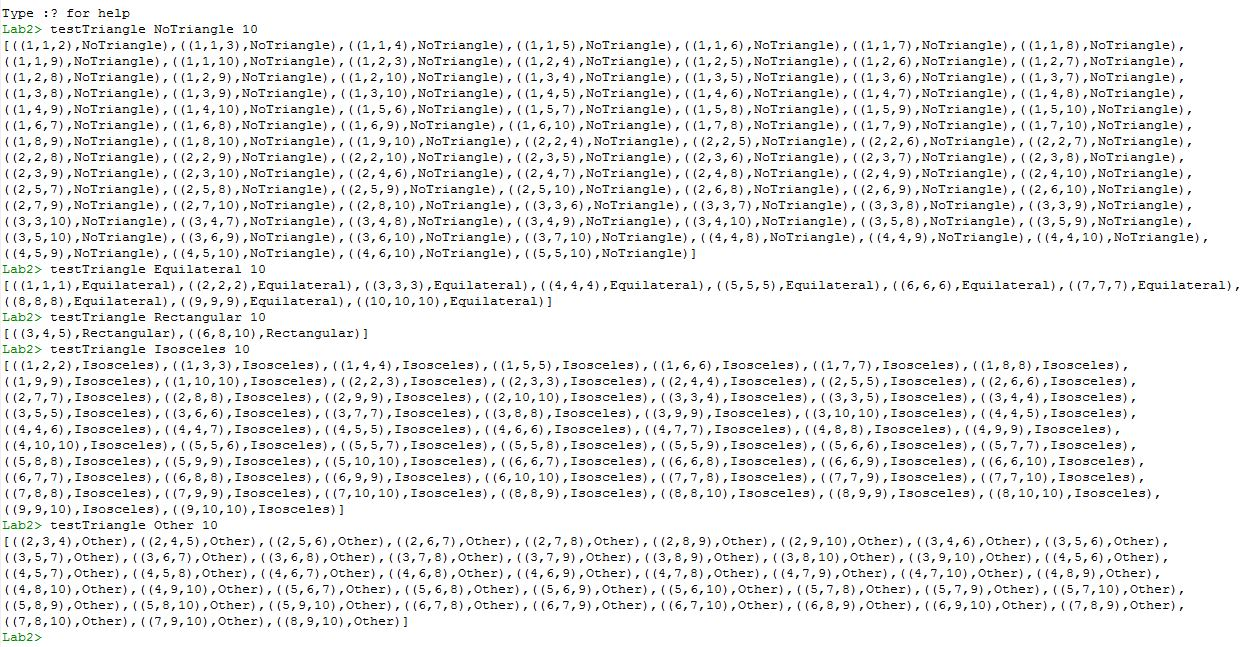
\includegraphics[scale=0.58]{Knipsel}

\section*{ Logic}

\begin{code}
contradiction :: Form -> Bool
contradiction f = not (satisfiable f)

tautology :: Form -> Bool
tautology f = all (\ v -> eval v f) (allVals f)

entails :: Form -> Form -> Bool
entails a b = all (\ v -> eval v f) (allVals f) where f = (Impl a b)

equiv :: Form -> Form -> Bool
equiv a b = all (\ v -> eval v f) (allVals f) where f = (Equiv a b)

\end{code}

XXX

\section*{Conjunctive Normal Form (CNF)}

\begin{code}
-- Precondition: Form is arrowfree and in negative normal form
-- Postcondition: Form is in conjunctive normal form
cnf :: Form -> Form
cnf (Prop x)		= Prop x
cnf (Neg (Prop x))	= Neg (Prop x)
cnf (Cnj f)		= Cnj (map cnf f)
cnf (Dsj [f, g])	= dist (cnf f) (cnf g)
cnf (Dsj (f:fs))	= dist (cnf f) (cnf (Dsj fs))

-- Precondition: Forms are in conjunctive normal form
-- Postcondition: Form is the the conjuctive normal form of (form1 v form2)
dist :: Form -> Form -> Form
dist (Cnj fs) g 	= Cnj (map (dist g) fs)
dist f (Cnj gs)		= Cnj (map (dist f) gs)
dist f g 		= Dsj [f,g]

\end{code}

In order to define test cases arbritrary formulas need to be defined first and converted to conjunctive normal form manually. In the workshop four functions were defined and converted to CNF therefore these four functions will be used to test our CNF. 
The four test cases are:

\begin{code}
test1 = Neg( Neg (Neg p))
test2 = Neg( Dsj[ p, Neg q])
test3 = Neg( Cnj[Neg p , Neg q])
test4 = Equiv (Impl p q) (Impl (Neg q) (Neg p))
\end{code}

The results are stated in the picture below and are verified by hand.

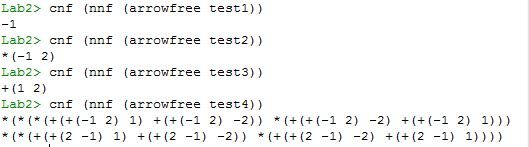
\includegraphics{Knipsel2}

To get the supplied formula to match with the pre-condition for 'cnf', we chain the 'arrowfree' and 'nnf' functions from Week2.hs:
\textbf{arrowfree}
\begin{description}
  \item[Pre-condition] \hfill \\
  Any formula.
  \item[Post-condition] \hfill \\
  A formula with the arrows (-> and <==>) replaced with disjunctions.
\end{description}

\textbf{nnf}
\begin{description}
  \item[Pre-condition] \hfill \\
  Arrow free formula.
  \item[Post-condition] \hfill \\
  Negative normal form of the arrow free formula.
\end{description}
The combination of 'arrowfree' and 'nnf' gives us a pre-condition where any formula can be used and a post-condition of an arrow free, negative normal formula which is what we need in our 'cnf' function.

\end{document}